Nowadays, mobile phones have dedicated processors to support video processing. This embedded streaming processor consumes tens of pJ per operation (pJ/op) and the battery capacity is only sufficient for playing video applications for a few hours \cite{simd}.
Furthermore, embedded systems like mobile devices have to run high performance applications like video encoding/decoding, wireless signal processing and 3D processing \cite{dongrio1}. These kind of devices often have a limited energy source, and because it is a handheld device, heat produced by power dissipation is another concern. For these reasons, energy efficiency is becoming the bottleneck in the design of such embedded systems.

In general, it is important to improve both performance and energy efficiency. The Very Long Instruction Word (VLIW) architecture is one example architecture designed to improve performance by executing multiple instructions in parallel, exploiting a program's Instruction Level Parallelism (ILP). By exploiting parallelism, the processor requires less cycles to do the same amount of work, thereby improving performance. 

The Transport Triggered Architecture (TTA) is similar to the VLIW architecture. However, instead of packing the operations in a single instruction, TTAs pack multiple transports in a single instruction \cite{tta}. For traditional VLIWs, each Register File (RF) is connected to every Function Unit (FU). Unlike VLIW, TTAs do not require that each FU has their own private connections to the RFs. Instead, an FU is connected to the RF by means of an interconnect. Another advantage that TTA has over VLIW is that it has explicit datapaths. With explicit datapaths, software bypassing is possible. The compiler can eliminate some RF accesses, which improves energy efficiency.

%TODO: Make link between explicit bp and compiler support.

Image and video processing applications typically have a high amount of Data Level Parallelism (DLP). The advantage of the Single Instruction Multiple Data (SIMD) architecture is that it naturally exploits DLP by processing multiple operations in parallel instead of processing them sequentially. Therefore, the same performance can be achieved at a much lower clock frequency, thereby reducing energy consumption \cite{dongrio1}. Furthermore, the instruction fetch and decode energy is shared amongst the processing elements. This improves energy efficiency with respect to an architecture that has an instruction fetch and decode for each processing unit, e.g. VLIW. A common bottleneck to achieve even higher energy efficiency with SIMD are the register files that consume a large amount of energy every time they are accessed. This work focusses on improving the energy efficiency by reducing accesses to the register files.

The proposed SIMD architecture has many processing elements that each have their own register file. This sums up to many register files that consume around 34.6\% of the total energy consumption \cite{dongrio1}. To further reduce energy consumption, we add explicit bypassing on top of the SIMD in order to eliminate some RF accesses. Adding explicit bypassing on top of the SIMD architecture resembles the TTA. Namely SIMD with explicit bypassing has an explicit datapath, like TTA also has an explicit datapath.

In the past, a compiler for the proposed architecture has already been implemented. This compiler exploits explicit bypassing \cite{dongrio1} and can compile a subset of OpenCL and C code \cite{dongrio2}. However, this compiler has a custom backend, and in order to standardize and improve maintainability, we want to use a compiler framework that supports our needs. To this end we use the LLVM framework to design and build a compiler for the proposed SIMD architecture.

%%%%%%%%%%OTHER PROEJCTS IN THIS SIMD, INCOMPLETE NOT CONTRIBUTING......
%This master project is part of a bigger project in which we work on the architecture and its compiler. There is another master's project going on about writing a compiler for the proposed SIMD architecture using the LLVM framework \cite{liu_zhenyuan}. However, this compiler focusses on vector instructions and does not support explicit bypassing. Therefore, we will focus on adding explicit bypassing on top of the new compiler. Furthermore, the proposed SIMD architecture is designed to be configurable. Another master's project will investigate in how to generate hardware code for different combinations of parameters.% \cite{boyan_liang}.

In the remainder of this chapter, first the target SIMD architecture is discussed in Chapter \ref{sec:simd}. Then we will introduce the reader to the LLVM compiler framework in Chapter \ref{sec:llvm}. We will give a more concrete statement of the problem in Chapter \ref{sec:problem_statement}. Finally, we will give an overview of the remainder of this report in Chapter \ref{sec:overview}.

\section{The SIMD Processor Architecture}\label{sec:simd}
The advantage of the SIMD architecture is that multiple operations are processed in parallel instead of processing them in a sequence. Therefore, the same performance can be achieved at a much lower clock frequency, thereby reducing voltage and thus energy consumption \cite{dongrio1}. Furthermore, because each Processing Element (PE) executes the same instruction, the Instruction Fetch (IF) and Instruction Decode (ID) can be shared amongst the PEs, reducing energy consumption.

We propose a wide SIMD architecture \cite{simd} that performs wide vector operations that exploit DLP by executing the same instruction on multiple data simultaneously. Figure \ref{fig:simd_overview} shows a general overview of the SIMD processor.
We have one Control Processor (CP) responsible for scalar operations and control flow i.e. jump/branch instructions. Furthermore, there is a wide array of PEs responsible for processing vector operations. The CP executes in parallel with the PEs, exploiting ILP.

\begin{figure}[H]
\centering
\includegraphics[width=.6\textwidth]{figures/simd_overview}
\caption{General overview of the wide SIMD architecture.}
\label{fig:simd_overview}
\end{figure}

The proposed architecture has a Reduced Instruction Set Computer (RISC) Instruction Set Architecture (ISA) that is divided up into three categories of instructions. In general, instructions have two operands and a destination register. Instructions that take two register files as operands are Register-type (R-type) instructions. Instructions that take a register file and an immediate as operands are called Immediate-type (I-type). The control flow can be controlled by using Jump-type (J-type) instructions, which can only be executed by the CP.

As an extra challenge for the compiler, the architecture is designed to be configurable, e.g. width of the PE array, bit width of the wires and registers, the number of stages that the instruction pipeline consists of, and whether it has implicit or explicit bypassing, can be configured. The data width of the wires and registers can be configured into 16-bits or 32-bits.

In order to support a configurable number of PE elements, a neighbourhood network topology is chosen for its scalability. With a circular neighbourhood network topology, the connection between the first and last PE does not introduce extra long wires, because the PEs can be placed in a circular manner \cite{dongrio2}.

%=============================== NN speech ===============================
%\section{Neighbourhood Network}\label{sec:nn}
%Each processor (CP or PE) does not only execute independently, but can also exchange data with its direct neighbours. However, because we have limited connectivity, moving data from one PE to another PE can introduce additional cycles. Namely, when communicating with non-direct neighbours. The circular neighbourhood network that is used to connect the processors is illustrated in Figure \ref{fig:neighborhood_network}. The CP can select data from the first and last PE, and each PE can communicate with its direct neighbours, or (not illustrated in Figure \ref{fig:neighborhood_network}) receive data from the CP by means of a broadcast.

%\begin{figure}[H]
%\centering
%\includegraphics[width=.4\textwidth]{figures/neighborhood_network}
%\caption{Illustration of the circular neighborhood network.}
%\label{fig:neighborhood_network}
%\end{figure}

%The processor selects data from its neighbours in the instruction decode stage. Depending on the "select data" bits, it either takes data from one of its neighbours or from itself. Table \ref{table:select_data} gives an overview of the communication mode, depending on the value of "select data". The "select data" bits are decoded in each instruction, as we will show in Chapter \ref{sec:isa}.
 
% \begin{table}[H]
%\caption{Communication model for the CP and PEs, depending on the value of "select data".}
%\begin{center}
%\begin{tabular}{|c|c|c|}
%\hline
%\textbf{select data} & \textbf{CP} & \textbf{PE} \\ \hline
%2'b00 & Select data from \emph{self}. & Select data from \emph{self}. \\ \hline
%2'b01 & Select data form \emph{last} PE. & Select data from \emph{right} neighbour. \\ \hline
%2'b10 & Select data from \emph{first} PE. & Select data from \emph{left} neighbour. \\ \hline
%2'b11 & Not used. & Select data from CP \emph{broadcast}. \\ \hline
%\end{tabular}
%\end{center}
%\label{table:select_data}
%\end{table}%

%The processors communicate with each other by writing directly to the output of the operand register based on the values of bits "select data" bits. When the value of these two bits is $00$, data is selected from the processor itself. When these bits are $01$, data is selected from the last PE, in case of the CP executing this instruction, and from the right neighbour in case of a PE executing this instruction. Similarly, having a value of $10$, data is selected from the first PE in case of the CP executing this instruction, or left neighbour in case of a PE is executing this instruction. Finally, a value of $11$ will select data from the CP broadcast in the case that a PE is executing the instruction.

%=============================== Datapath speech ===============================
\subsection{Processor Pipeline and Datapath}\label{sec:processor}
%TODO: Write new paragraph about.general layout
\begin{figure}[t!]
\centering
\includegraphics[width=.5\textwidth]{figures/4-stage_bypass}
\caption{4-stage pipeline processor overview.}
\label{fig:4_stage}
\end{figure}

\begin{figure}[b!]
\centering
\includegraphics[width=.5\textwidth]{figures/5-stage_bypass}
\caption{5-stage pipeline with processor overview.}
\label{fig:5_stage}
\end{figure}

Generally, each processor (CP or PE) has its own registers and three functional units, i.e. ALU, MUL and LSU. 

The instruction pipeline is divided up into four or five stages. Top down, we have an IF-stage, an ID-stage, one or more execution stages and a Write Back (WB) stage. The architecture shown in Figure \ref{fig:4_stage} has four stages while the architecture shown in Figure \ref{fig:5_stage} has five stages.

The neighbourhood communication network is implemented by overriding the output of $operand\ 1$ in ID-stage. Depending on the decoded instruction, data is either selected from another (neighbouring) processor, from the local RF or from the bypass network. Each FU has private input registers, which keep the result at the output of a compute unit valid as long as no new operation or input is assigned to it \cite{dongrio1}. The outputs can be used in the bypass network to bypass any of the operands in an instruction. This \emph{operand isolation} reduces toggling in the FUs, and creates extra opportunities for bypassing.

We can configure the SIMD to have either explicit or implicit bypassing. With implicit bypassing, also called transparent bypassing it is the hardware's responsibility to handle bypassing. With explicit bypassing, on the other hand, the bypasses are encoded in the instructions, and it is thus the compiler's responsibility to handle bypassing.

\begin{figure}[t]
\centering
\subfloat[Datapath with implicit bypassing.]{\includegraphics[width=.35\textwidth]{figures/transparent_bypass}%
\label{fig:transparent_datapath}}
\hfil
\subfloat[Datapath with explicit bypassing.]{\includegraphics[width=.35\textwidth]{figures/explicit_bypass}%
\label{fig:explicit_datapath}}
\caption{Bypassing network differences between implicit bypassing and explicit bypassing.}
\label{fig:datapath_approaches}
\end{figure}

%We can configure the SIMD to have four or five stages. With four stages shown in Figure \ref{fig:4_stage}, all instructions take a single cycle, while with the five stages shown in Figure \ref{fig:5_stage}, ALU takes a single cycle, while MUL and LSU take two cycles, as shown in Table \ref{table:FU_cycles}. With 5 stages, MUL takes twice as many cycles. However, additions are simpler to perform, therefore the efficiency. 

%\begin{table}[H]
%\caption{Cycles per FU.}
%\begin{center}
%\begin{tabular}{|c|c|c|}
%\hline & \multicolumn{2}{c|}{\textbf{Cycles}} \\ \hline
%\textbf{FU} & \textbf{4-stage} & \textbf{5-stage} \\ \hline
%ALU & 1 & 1 \\ \hline
%MUL & 1 & 2 \\ \hline
%LSU & 1 & 2 \\ \hline
%\end{tabular}
%\end{center}
%\label{table:FU_cycles}
%\end{table}%

\begin{table}[b]
\caption{Special purpose registers.}
\begin{center}
\begin{tabular}{@{}l l@{}}
\toprule
\textbf{Register} & \textbf{Purpose} \\ \hline
\emph{r0} & Constant value zero. \\
\emph{r1} & PE\_ID (PE only). \\
\emph{r3} and \emph{r4} & Return value registers. \\
\emph{r5} through \emph{r8} & Argument passing. \\
\emph{r9} & Link register (CP only). \\ 
\emph{r10} & Frame pointer. \\
\emph{r11} & Stack pointer. \\
%\multicolumn{2}{|l|}{Only with \emph{explicit bypassing}:} \\ \hline
%$R_{27}$ & $BP\_src27$ (5 stages only). \\ \hline
%$R_{28}$ & $BP\_src28$. \\ \hline
%$R_{29}$ & $BP\_src29$. \\ \hline
%$R_{30}$ & $BP\_src30$. \\ \hline
%$R_{31}$ & $BP\_src31$. \\ \hline
\bottomrule
\end{tabular}
\end{center}
\label{table:special_registers}
\end{table}%

%The main difference between the two approaches is that where transparent bypassing always performs a write to a register, this is optional for explicit bypassing, as we will show in Chapter \ref{chapter:software_bypassing}.
One of the advantages of explicit bypassing is that certain writes to a register can be avoided. Namely, when the result of an instruction is bypassed and not used anywhere else, we do not need to store it in a register because we would never read it. Avoiding writes to the RF reduces the total energy consumption. Since there are many register files in a wide SIMD, reducing the energy consumption of the register file has a large impact on the overall energy consumption \cite{dongrio1}. Because of this, reducing the register file's energy consumption is of great importance. Furthermore, the explicit data path shown in Figure \ref{fig:explicit_datapath} has two extra sources compared to the transparent data path in Figure \ref{fig:transparent_datapath}. These additional bypass sources increase the chance that a result is being bypassed. In the explicit bypassing version, bypassing sources are directly accessible by the instruction. This is done by reserving part of the RF address space for the bypass sources. The disadvantage of this is that the register index space is reduced, however, we do not have to change the instruction format in order to specify that an operand of an instruction is bypassed from a previous instruction.

The total number of registers grows linearly with the number of PEs because each processor has 32 registers. With a wide SIMD, we, therefore have many registers that in total consume a considerable amount of energy, namely 34.6\% of the total energy consumption \cite{dongrio1}. Some of these registers have a special purpose, e.g. register $R_0$ is connected to ground is has a static value of $0$, these are shown in Table \ref{table:special_registers}.


%Todo: change this picture to have explicit and implicit bypassing instead. State then that we will be focussing on explicit bypasisng.



%Todo: add small example, having on one side normal ops. On the other hand haing implicit bypassing and finally explicit bypassing (without the store).

%\begin{figure}[b!]
%\centering
%\subfloat[4-stage pipeline with explicit datapaths.]{\includegraphics[width=.4\textwidth]{figures/4-stage_bypass}%
%\label{fig:4stage}}
%\hfil
%\subfloat[5-stage pipeline with explicit datapaths.]{\includegraphics[width=.34\textwidth]{figures/5-stage_bypass}%
%\label{fig:5stage}}
%\caption{The pipeline of the SMD processor architecture with explicit datapaths.}
%\label{fig:pipeline_stages}
%\end{figure}

%%=============================== instruction format speech ===============================
%\section{Instruction Format}\label{sec:isa}
%%Change (optional)
%%% namely, one scalar and one vector instruction.
%%With
%%% namely, one scalar instruction that is executed on the CP, and one vector instruction that is executed on each of the PEs.
%Similar to a 2-issue VLIW instruction, an SIMD instruction consists of two subinstructions. An SIMD instruction is a 56-bit instruction that is divided up in two 28-bit subinstructions, namely, a scalar and a vector instruction. Only the CP can perform jump and branch instructions, therefore, the vector instruction can be either a R-type or an I-type instruction, while a scalar instruction can be a R-type, I-type or J-type instruction. Both sub instructions have a format, as shown in Figure \ref{fig:instruction_format}.

%\begin{figure}[H]
%\centering
%\includegraphics[width=\textwidth]{figures/instruction_format}
%\caption{Generic overview of the instruction format.}
%\label{fig:instruction_format}
%\end{figure}

%There are two guard bits $p1$ and $p2$, that can be set by using a set flag instruction. Consequently we can them for predicate execution. The instructions, branch if flag (not) set and conditional move read the predicate flag before executing. For the full overview of supported instructions, see Appendix \ref{chapter:supported_operations}.

%Note that the "select data" bits are also part of the instruction as we explained in Chapter \ref{sec:nn}. The CP and PEs can communicate by setting these bits. The communication model is shown in Table \ref{table:select_data}.


\section{The LLVM Compiler Framework}\label{sec:llvm}
The LLVM project was started in 2000 by Chris Lattner, as a research project at the University of Illinois with the goal of providing a modern, Static Single Assignment (SSA)-based compilation strategy capable of supporting both static and dynamic compilation of arbitrary programming languages. It was first released in 2003 and the project has grown rapidly since then. It has become popular amongst major companies, e.g. Google, Apple, and Sony, for its powerful multi-stage compilation strategy and outstanding extendibility. LLVM is a collection of modular and reusable compiler and toolchain technologies. Generally, LLVM follows a 3-phase design, which is divided between a frontend, a code independent optimizer and a backend, illustrated in Figure \ref{fig:3phase_design}.

\begin{figure}[H]
\centering
\includegraphics[width=.7\textwidth]{figures/3phase_design}
\caption{3-phase design: frontend, optimizer and backend.}
\label{fig:3phase_design}
\end{figure}

%Reorder list: [IR, Lexical analysis, Syntax analysis, ]
\textbf{The frontend} is responsible for translating code of an arbitrary programming language into LLVM's Intermediate Representation (IR) code. The LLVM instruction set represents a virtual architecture that captures the key operations of ordinary processors, but avoids machine specific constraints such as physical registers. Instead, it has an infinite amount of virtual registers in SSA form, which means that each virtual register is assigned only once and each use of a variable is dominated by that variable's definition. This simplifies the data flow optimizations because only a single definition can reach a particular use of a value, and to find that definition is trivial \cite{llvm_strategy}.
%frontend talk, straight from the Dragon Book plz.
%introduce parser and lexical analysis and that it is kept in an AST, which will be translated as a final step to IR.
%Perhaps an example?
%TODO: rewrite first sentence in my own words.
In the first phase of a compiler, the main task of the lexical analyzer is to read the input characters of the source program, group them into luxemes, and produce as output a sequence of tokens. These tokens are used by the parser for syntax analysis, where it is verified that the sequence of tokens can be reconstructed according to the syntax of the input language. The parser reports any syntax errors during this process and should be able to recover from the error in order to continue processing the rest of the program. The parser constructs a parse tree, and the semantic analyzer uses this parse tree to check for consistency with the language definition. Type checking is also done during this stage, and the information is kept in a syntax tree. The result of these phases is an Abstract Syntax Tree (AST) of the program, which can be translated into three-address IR code. %We will discuss LLVM's IR in more detail in Chapter \ref{sec:ir}

\begin{figure}[b!]
\centering
\includegraphics[width=.7\textwidth]{figures/frontend}
\caption{Overview of the components that the frontend compromises.}
\label{fig:frontend}
\end{figure}

\textbf{The optimizer} contains a collection of analysis and semantic-preserving transformations that can be used to optimize IR code. One of the advantages of LLVM is that when you build a new backend for any given processor architecture you immediately have access to all of these optimizations. Below we give some of these optimizations that are explained more detailed in the literature \cite[Chapter~9]{dragon_book}.%TODO: provide chapter in cite.
\begin{itemize}
\item \emph{Constant propagation} computes for each point and each variable in the program, whether that variable has a unique constant value at that point. This can then be used to replace variable references with constant values.
\item \emph{Constant folding} recognizes and evaluates constant expressions at compile time rather than runtime. For example, `$add\ 1+2$' can be replaced by `$3$'. Statements like `$add\ 1+2$' can be introduced by other optimizations, e.g. constant propagation. 
\item \emph{Common sub-expression elimination} recognizes that the same expression appears in more than one place, and that performance can be improved by transforming the code such that the expression appears in one only place.
\item \emph{Copy propagation} replaces each target of a copy statement with that of the copied value. For example, if we have a copy statement, $x = y$. Then the uses of $x$ can be replaced by $y$. Some optimizations require that this optimization is performed afterward to clean up, e.g. common sub-expression elimination requires this pass to run afterward. 
\item \emph{Dead code elimination} removes code that does not affect the program's results. This avoids executing irrelevant operations and reduces the code size of a program.  
\item \emph{Loop invariant code motion} aims at moving code that is independent of the loop iteration out of the loop body. It does this by moving the loop independent statement above the loop, saving it in a temporary variable, and use it in each iteration of the loop. Now the loop independent statement is computed only once instead of every iteration. 
\item \emph{Function inlining} verifies whether inlining functions in its callees gives a performance benefit. If doing this would give a performance benefit, it replaces the call to the function with the function body. This optimization often is useful for small functions because it reduces the overhead that is introduced when a function call is made, e.g. storing frame pointer, storing function parameters and jump to the code to where the function is defined.     
\end{itemize}

\begin{figure}[t]
\centering
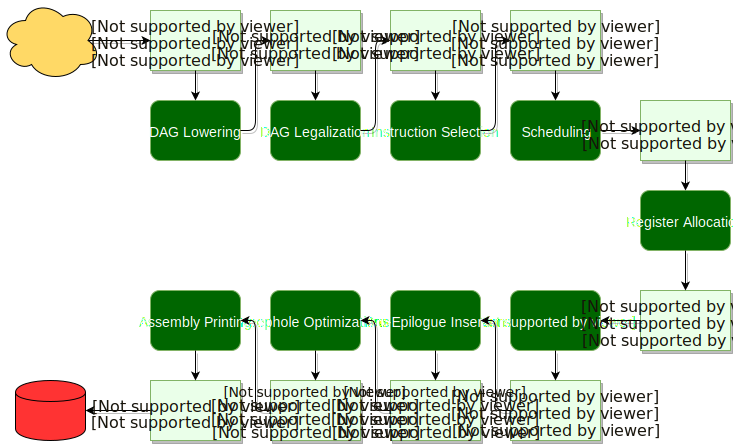
\includegraphics[width=.85\textwidth]{figures/code_generation_sequence}
\caption{Code generation sequence, from LLVM code to assembly code.}
\label{fig:code_generation}
\end{figure}

%TODO: apply following namings: Instruction, Machine instruction, scheduled instruction in SSA form, schedule instruction not in SSA form.
\textbf{The backend} translates, according to a processor architecture, IR code to a target specific assembly language. It does this by going through a sequence of code generation stages, illustrated in Figure \ref{fig:code_generation}. The rectangular boxes indicate the data structure that is used by and produced by a given stage, and the name of each stage is denoted in a rectangular box with rounded corners. During this process, first, the IR code is lowered to a Directed Acyclic Graph (DAG) in which each node represents one instruction. However, for some architectures, not all data types and instructions are supported. For this reason, the DAG is legalized to something that is supported by the target architecture. Instruction selection maps each of the nodes into machine nodes, by matching patterns. %After that, the instruction selector maps the pattern of LLVM code into the target machine code and builds a new DAG whose nodes represents the target instructions.
Then we have a DAG consisting of only target specific machine instructions, in SSA form. Having naive machine instructions, the next step is to schedule them. We schedule the machine instructions according to the resource information of the target processor and assign each instruction to a specific cycle. 
%We will discuss scheduling in more detail in Chapter \ref{sec:scheduling}. 
Now the instructions are represented in a list rather than a DAG, but still in SSA form. The Register Allocator (RA) then assigns physical registers to each of the virtual registers, now the list is not in SSA form. 
%We will discuss RA in more detail in Chapter \ref{sec:register_allocation}. 
The post-allocation pass can improve the schedule, taking the physical registers and register pressure, that is known at this point, into account. After that, some epilogue and prologue code might need to be inserted, e.g. saving/restoring the caller/callee registers and reserving/destroying of the function's stack frame. Peephole optimizations are target specific improvements to the schedule that has been constructed. These optimizations deal with very specific optimizations that can only be done at the end of the process. Finally, the assembly printer prints the assembly code.
%backend talk -> huuge



%\subsection{Instruction Scheduling}\label{sec:scheduling}
%After instruction selection, the program is represented in SSA form as a DAG. Each instruction is represented as a $MachineSDNode$ in a $MachineBasicBlock$. After scheduling has been performed, each instructions now is represented as a $MachineInstr$. 



%ach instruction is scheduleDuring instruction schdduling, each $MachineBasicBlock$ is scheduled by the scheduler and transformed into a $MachineInstr$. After this phase, instructions are represented as $MachineInstr$.

%\subsection{Register Allocation}\label{sec:register_allocation}
%Register allocation is executed during the code generation phase and consists of finding a mapping of a program with an unlimited number of virtual registers to a program with a limited number of physical registers.
%Examples, machine instrs on the left in SSA form, on the right with proper registers next to it.
%Introduce at least 

\subsection{Scheduling and Register Allocation}\label{sec:scheduling_and_ra}
From a compiler's perspective, certain instructions address memory locations. \emph{Store} instructions access the memory to put the value of a register into memory at a certain location, addressable by its address. \emph{Loads}, on the other hand load a value from a location in memory to a register. Other instructions calculate a result of an operation and stores the result in a register. Operations that store the result in a register, or load a value from memory into a register, actually define a register. Before scheduling and register allocation, the sequence of instructions contain an unlimited number of virtual registers and the instructions are in a DAG that preserves all control flow and data dependencies. Data dependencies are ordering constraints that influence the order of execution. Typically, there are three kinds of data dependencies \cite{data_dependece}:
\begin{enumerate}
\item There is a Read-after-Write (R/W) dependency, also called a \emph{flow dependence} from operation $a$ to $b$ if $a$ defines a register that is used by $b$.
\item  There is a Write-after-Read (W/R) dependency, also called an \emph{anti-dependency} if for operations $a$ and $b$, we have that $a$ uses a register that is redefined by $b$. 
\item There is a Write-after-Write (W/W) dependency, or \emph{output dependency} from $a$ to $b$ if $a$ defines a register that is redefined by $b$.
\end{enumerate} 
Flow dependencies are also known as \emph{true dependencies} and anti and output dependencies as \emph{false dependencies}, introduced by register allocation. While in SSA form, each variable is defined exactly once, we have only true dependencies in that form. After register allocation where we assign physical registers to each virtual register, we may assign a physical register to multiple virtual registers, see Listing \ref{lst:ra_example}. This process introduces false dependencies and can often be resolved with renaming techniques \cite{renaming}. 

\begin{center}
%TODO: include a data dependency graph for the example below
\captionof{lstlisting}{Redefining physical registers by assigning them to multiple virtual registers.}
\begin{minipage}[t]{.4\textwidth}
\begin{lstlisting}
add <@\textcolor{red}{\%v1}@>, %src1, %src2
add <@\textcolor{red}{\%v2}@>, %src2, %src3
add %v3, <@\textcolor{red}{\%v1}@>, <@\textcolor{red}{\%v2}@>
add %v4, %sp, 4
\end{lstlisting}
\end{minipage}
\begin{minipage}[t]{.4\textwidth}
\begin{lstlisting}
add <@\textcolor{red}{r1}@>, r5, r6
add <@\textcolor{red}{r2}@>, r6, r7
add <@\textcolor{red}{r2}@>, <@\textcolor{red}{r1}@>, <@\textcolor{red}{r2}@>
add <@\textcolor{red}{r1}@>, r8, r9
\end{lstlisting}
\end{minipage}
\label{lst:ra_example}
\end{center}

%TODO: add control flow dependecy explanation, optionally from Code Generation for TTAs p.

Sometimes there are not enough registers available to allocate a physical register to all virtual registers because there are only a limited number of physical registers available. In that case, register \emph{spilling} may be necessary to free one or more registers by storing them in the stack. Then consequently you are required to retrieve them from the stack right before they are needed.

%TODO: insert general RA algorithms and heuristics. Graph colouring, and use this reference \cite{ra}.
There are multiple register allocators available in LLVM, e.g. basic, fast, greedy and Partitioned Boolean Quadratic Problem (PBQP) register allocation. PBQP is a nearly optimal approach that does register allocation in phases, i.e. spilling, register assignment and copy coalescing. After spilling, RA can be done in polynomial time, but copy coalescing is NP-complete \cite{pbqp}. The other three register allocators are linear scan based algorithms that use heuristics and visit live ranges in order, although it is possible to implement a custom register allocator.

%TODO: insert scheduling talk, including algorithms, heuristics and LLVMs available schedulers.

A common problem in compilers is the ordering in which to do scheduling and register allocation. If registers are allocated before scheduling, the resulting code tends to have many storage dependencies that limit code scheduling. On the other hand, if the code is scheduled before register allocation, the schedule created may require so many registers that register spilling is required, which may negate the advantages of instruction-level parallelism (ILP) \cite[Chapter~10.2.4]{dragon_book}. Whether to do register allocation first, or scheduling first, or to address these problems at the same time is often referred to as, phase-ordering problem. 

In general, you can solve scheduling exactly using algorithms, e.g. integer programming or constraint programming, or one can solve the problem, but without guaranteeing that an optimal solution is found using heuristics. With LLVM there are two main schedulers, i.e. list scheduler and Machine Instruction (MI) scheduler that use heuristics to find a solution, although it is possible to implement a custom scheduler for an architecture at hand. 

%Problem statement -> incorporate Roel's Feedback..!!!
\section{Problem statement}\label{sec:problem_statement}
An SIMD architecture has been designed and a legacy compiler exists. However, the legacy compiler is too custom and therefore difficult to maintain. Many optimizations still have to be implemented. One of the advantages of LLVM is that a large community works on it. Many optimizations are already in place and can immediately be used for our compiler. Standardizing and having proper tool support improves maintainability of the compiler. %Namely, anyone familiar with LLVM can now understand and improve the compiler.
For this reason, a new compiler is being implemented in LLVM.

We have a new compiler in LLVM that supports vector operations and can compile any IR code into SIMD specific assembly. The legacy compiler does have support for explicit bypassing. We want to develop explicit bypassing in the new compiler structure.

The goal of this project is therefore to generate efficient code to support explicit bypassing. We have separated the goal in multiple research questions:

\begin{enumerate}
\item How do we implement explicit bypassing within LLVM?

How does this fit in the new compiler.
\item What alternative approaches are there to implement it?

Do we do this in an early stage, or at a later stage in the compiler.
\item How do we know which approach is more efficient?

What metric would be suitable to evaluate the different approaches with each other and with the legacy compiler.
\end{enumerate}



%Deelvragen:
% - Hoe impl. ik expl. in LLVM
% - Wat zijn de stappen
% - Alternatieven aanpakken
% - Hoe weet ik welke beter is
% - Hoe is dat nuttig voor andere architecture


%Overview
\section{Overview}\label{sec:overview}
In the remainder of this report we will discuss related works in Chapter \ref{chapter:related_work}. We will discuss bypassing, and show the difference between implicit and explicit bypassing in Chapter \ref{chapter:explicit_bypassing}. Proposed solutions for how to achieve our goal will be discussed in Chapter \ref{chapter:solutions} and we will discuss on how to evaluate each of the proposed solutions in Chapter \ref{chapter:evaluation}. Preliminary conclusions are given in Section \ref{chapter:conclusions} and we will provide a planning for this master thesis in Chapter \ref{chapter:planning}.